\documentclass[12pt]{article}
\usepackage{graphicx}
\usepackage{epstopdf}
\usepackage{url}
\usepackage{color}
\usepackage{caption}
\usepackage{subcaption}

\usepackage[margin=0.5in]{geometry}

\begin{document}
\title{\textbf{ECON 5P08 Project: Analysis of UK Balance of Payments, 1988-2018}}
\author{Zachary Mesic (5820105)}
\date{\today}
\maketitle

\thispagestyle{empty}
\vfill
\begin{center}
\textbf{BROCK UNIVERSITY}
\break
Master of Business  Economics
\break
Professor Katerina Koka
\linebreak
\linebreak
\textbf{\copyright{Zachary Mesic (5820105)}}\\
All rights reserved\\

2020
\end{center}

\newpage

\begin{flushleft}
\begin{abstract}
The purpose of this research project is to examine the behavior of the Balance of Payments of a particular country of our choosing. The country that I have chosen to observe is the United Kingdom. I collect data from two main databases:  \textit{OECD.stat} and the \textit{Office for National Statistics}. The data I obtain includes: GDP and components (expenditure), annual Current Account, Trade Balance, and NIIP(Net International Investmenrt Position) levels (aggregate and \% of output), and Bilateral Trade data with the UK's largest trading partners.
\break
\linebreak
The first section of this project offers a presentation of some of the general observations that can be made about the UK's Balance of Payments. The data are displayed in the form of time series that were all generated in RStudio (coding is included at the end). I provide some brief forecasting on some of the trends and why they might be taking place.
\break
\linebreak
The second section of the project outlines the different detrending methods that were used on the datasets. They include HP-filtering process, Log-Linear detrending, and Log-Quadratic detrending. The HP-filtering process was completed using an online HP-filter (website included in bibliography). Both Log-Linear and Log-Quadratic detrending were completed in RStudio through running a regression of logged variables on a trend variable \textit{t} (in LQ case, $ \textit{t} + \textit{t}^2$).
\break
\linebreak
Lastly, using the detrended components of GDP obtained from the Log-Quadratic detrending process, I provide some insight as to whether or not the behavior of UK Balance of Payments is consistent with the \textbf{Ten Facts about Business Cycles Around the World} introduced in 5P08 lecture. I find that the behavior of GDP components, when detrended using a LQ process, display identical behavior to that observed in the Ten Business Cycle Facts.
\break
\linebreak
\textbf{Keywords:} UK, GDP, Balance of payments, Current Account, Trade Balance, NIIP, time series, HP-filter, log-linear detrending, quadratic-log detrending, Business Cycles.
\end{abstract}
\end{flushleft}

\newpage

\tableofcontents

\newpage
\section{BoP Data: GDP, Current Account, Trade Balance, \& NIIP}

\subsection{GDP (expenditure approach)}

\begin{figure}[h!]
\centering
\begin{subfigure}{.5\textwidth}
  \centering
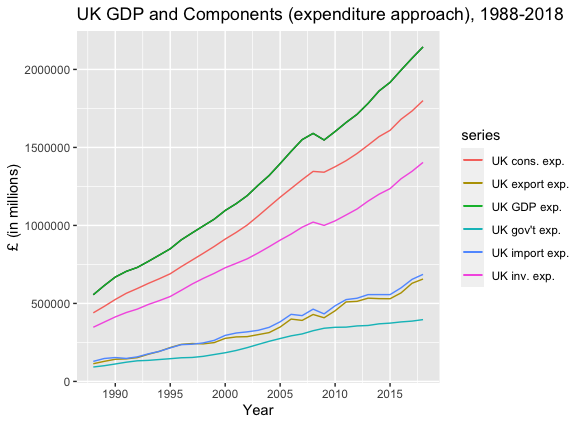
\includegraphics[scale=0.45]{1.png}
\label{}
\caption{UK GDP and Components (expenditure approach) \\ 1988-2018.}
\end{subfigure}%
\begin{subfigure}{.5\textwidth}
  \centering
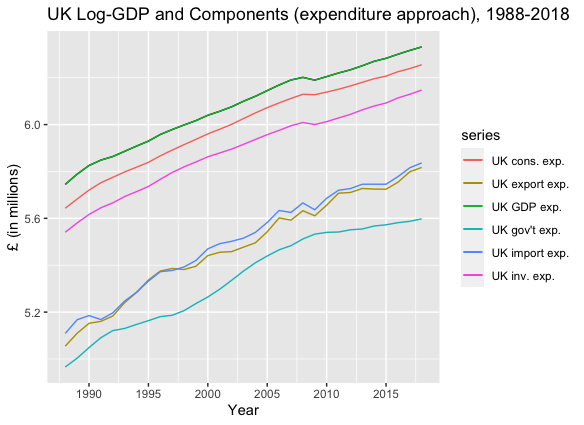
\includegraphics[scale=0.45]{1a.png}
\label{}
\caption{UK Log-GDP and Components (expenditure \\ approach), 1988-2018.}
\end{subfigure}
\end{figure}

\begin{flushleft}
The first variable that is observed is UK Gross Domestic Product over 1988-2018. The data for GDP was obtained using the \textit{OECD.stat} database and was specifically collected through the expenditure approach (\textbf{note: although the notes say to collect Real GDP per capita, I was unable to locate this data for the GDP components themselves in per capita terms. For consistency, I kept the measure of GDP the same as the components, which is all in aggregate expenditure form}). 
\break
\linebreak
As we can see, both GDP and log-GDP and its components are steadily incereasing over the designated time frame. This trend is consistent with other OECD countries in the world, and it even appears that there is an \textit{exponential} increase in aggregate GDP. The same can be said about consumption and investment components, while government expenditure, exports, and imports appear to be growing closer to a \textit{constant} rate.
\break
\linebreak
Some other observations include that both consumption and investment make up a greater portion of aggregate GDP than do the other components by a sginificant portion. It also appears that in the UK, government spending and level of exports move very closely with one another.
\end{flushleft}

\newpage

\subsection{Current Account, Trade Balance, \& NIIP}

\begin{figure}[h!]
\centering
\begin{subfigure}{.5\textwidth}
  \centering
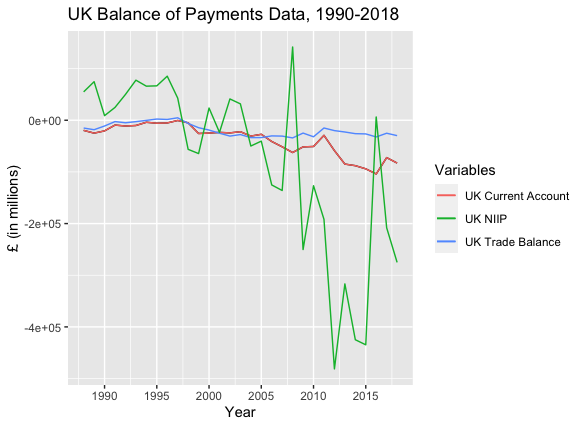
\includegraphics[scale=0.45]{2.png}
\label{}
\caption{UK Balance of Payments Data, 1990-2018.}
\end{subfigure}%
\begin{subfigure}{.5\textwidth}
  \centering
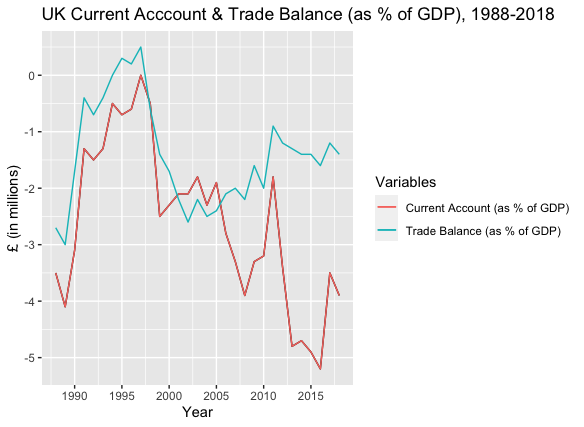
\includegraphics[scale=0.45]{3.png}
\label{}
\caption{UK Current Acccount \& Trade Balance (as \% of GDP), 1988-2018.}
\end{subfigure}
\end{figure}

The following variables that are observed include the Current Account, Trade Balance, and NIIP. The data for these variables was collected from the \textit{Office for National Statistics} database. I also include measures of the Trade Balance and Current Account in the form of \% of GDP. Both figures span over the designated time frame of 1988-2018.

\subsubsection{Current Account}

Starting with the Current Account, we see that there has been a gradual decrease since the late 1980s. Since the Current Account is indeed negative, this means that its net extrernal debt will increase. The net external debt steadily increases as is displayed in the figure above.

\subsubsection{Trade Balance}

The Trade Balance moves similarly to that of the Current Account. Although it is closer to being even (zero), it does appear to be in a very weak downward trend. A Trade Balance is defined as the difference between a countries net exports and its imports, or the sum of the goods and services balances. In this case, since the Trade Balance is negative, UK total imports exceed exports. This is confirmed in the aggregate data.

\subsubsection{NIIP}

Lastly, we observe the NIIP, or the Net International Investment Position. We can see, that along with the CA and TB, the NIIP is in a downward trend. However, it is important to note that the degree of fluctuation or volatility is much higher in the NIIP than it is in the CA and TB. We can also infer that the UK will not be able to run a perpetual Trade Balance deficit, given that its NIIP is negative. A negative NIIP implies that the UK is a net debtor. Therefore, it must eventually run a surplus in its Trade Balance in the future in order to finance its debt.

\newpage

\section{Bilateral Trade}

\subsection{Trade with Major Trading Partners}

\begin{figure}[h!]
\begin{center}
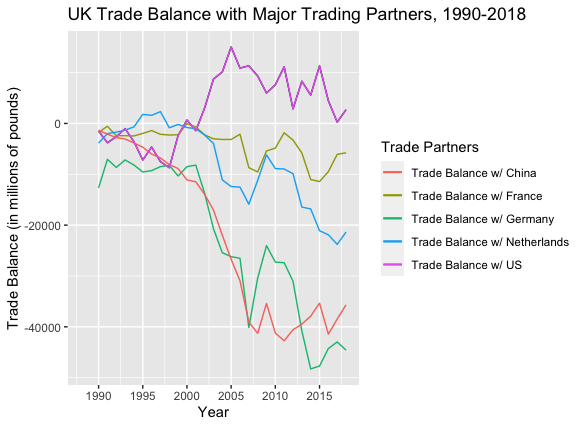
\includegraphics[scale=0.75]{5.png}
\label{}
\caption{UK Trade Balance with Major Trading Partners, 1990-2018.}
\end{center}
\end{figure}

\begin{flushleft}
This next section provides insight into the Bilateral Trade between the UK and its largest trade partners: China, France, Germany, the Netherlands, and the US. The data used in this section was collected from the \textit{OECD.stat} database. It specifically measures the Trade Balance of the UK between each respective country.
\break
\linebreak
When we observe the figure above, we can see that, with the exception of the US, the UK has a negative Trade Balance with all of its major trading partners. This means that the amount of goods and services that the UK imports from its major trading partners exceeds the amount of goods and services it exports to them.
\break
\linebreak
When we break it down by individual country, we see that UK's Trade Balance with France and the Netherlands are closer to zero, however are still constantly decreasing. The Trade Balance of the UK with Germany and China on the other hand is much more significantly negative, and appears to be increasingly downward in its trend.
\break
\linebreak
Finally, the UK appears to have a Trade Balance surplus with the United States. This indicates that the amount of goods and services that the UK exports to the US exceeds the amount of goods and services it imports from them.
\end{flushleft}


\newpage

\subsection{Trade with EU vs. non-EU Countries}

\begin{figure}[h!]
\begin{center}
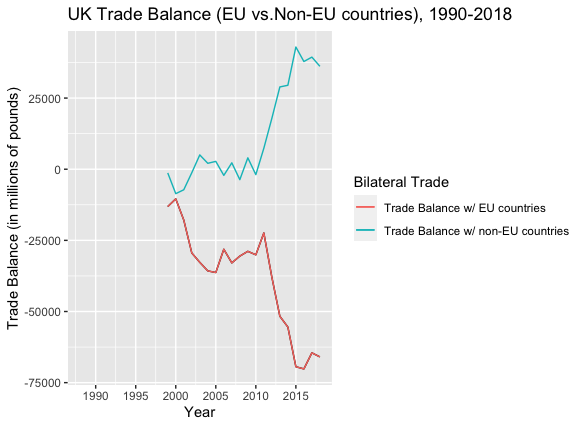
\includegraphics[scale=0.75]{4.png}
\label{}
\caption{UK Trade Balance (EU vs.Non-EU countries), 1990-2018.}
\end{center}
\end{figure}

\begin{flushleft}
The next figure displays the overall Trade Balance of the UK with countries in the European Union versus non-EU countries over 1999-2018. This data was collected fromthe  \textit{Offce of National Statistics} database. Althought time frame is incomplete (due to lack of available data) I felt that this would be an interesting graphic to include considering the recent political outcomes (\textbf{Brexit}) that will certainly have an impact on the country's  Balance of Payments.
\break
\linebreak
To begin, we can see that there is a Trade Balance deficit between the UK and the European Union and a Trade Balance surplus between the UK and non-EU countries. Given that prior to this year, Great Britian itself was a part of the EU, it makes sense that they would have a negative Trade Balance with other EU countries as the EU as a political/economic institution surely made it easier for the country to import goods and services from other members. However, there are also those who argue that the EU as an institution makes it more difficult for the UK to enact trade policies independent of the EU with other countries as well.
\break
\linebreak
It will be very ineresting to see whether or not these Trade Balances continue in their respective upward and downward trends. Perhaps they will reverse given UK's exit of the European Union as the impact on the BoP will surely be nonnegligible. 


\end{flushleft}

\newpage

\section{HP Filter Detrending}

In this section, I provide a brief summary of the various detrending methods that were completed on the following variables: Current Account, Trade Balance, GDP, consumption, investment government spending, net exports, and imports. The first detrending method adopted for this project is HP-filtering. I used an online HP-filter provided in the bibliography.

\subsection{Trade Balance and Current Account}

\begin{figure}[h!]
\begin{center}
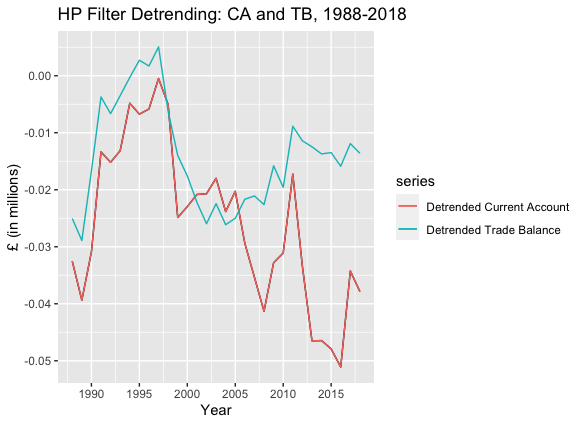
\includegraphics[scale=0.5]{hp2.png}
\label{}
\caption{HP Filter Detrending: CA and TB, 1988-2018.}
\end{center}
\end{figure}

\begin{flushleft}
The figure above displays detrended Current Account and Trade Balance for the UK over the period 1988-2018. Because their values are, for the most part, negative, they had to be detrended through dividing the variables by the exponential trend component of output, $exp(y_{t}^s)$. 
\break
\linebreak
We can see that, even when detrended, the Current Account and Trade Balance tend to move in the same direction with one another, with the Current Account experiencing slightly more volatile behavior.
\end{flushleft}

\newpage

\subsection{GDP and Components}

\begin{figure}[h!]
\centering
\begin{subfigure}{.5\textwidth}
  \centering
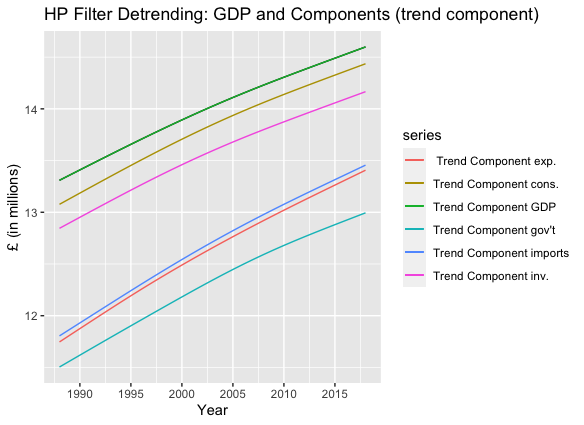
\includegraphics[scale=0.45]{hp1.png}
\label{}
\caption{HP Filter Detrending: GDP and Components \\ (trend component).}
\end{subfigure}%
\begin{subfigure}{.5\textwidth}
\centering
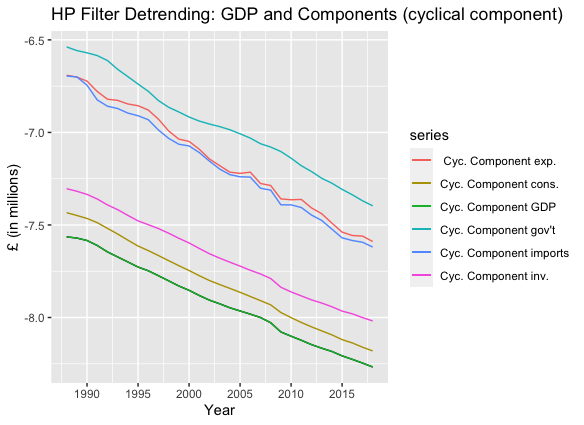
\includegraphics[scale=0.45]{hp3.png}
\label{}
\caption{HP Filter Detrending: GDP and Components \\ (cyclical component).}
\end{subfigure}
\end{figure}

\begin{flushleft}
The figures above display both the 'trend' and 'cyclical' components of the HP filtering process for GDP and its components. 
\break
\linebreak
When isolating for the trend component of GDP and its components, we can see that there is clearly a consistent upward trend taking place amongst all variables, with all of the curves adopting almost identical upward slopes.
\break
\linebreak
When isolating for the cyclical component, the results appear to be rather ambiguous. In other words, it is difficult to identify any cyclical behavior amongst GDP and its components when detrended using the HP filter.

\end{flushleft}

\newpage

\section{Log-Linear Detrending}

In this section, I provide a brief overview of the Log-Linear detrending method that was implemented in this project. The Log-Linear detrending process was completed in RStudio through running a regression of logged variables on a trend variable $t$, where $t \ \epsilon \ \{1,...31\}$.

\subsection{Trend Components}

\begin{figure}[h!]
\centering
\begin{subfigure}{.5\textwidth}
  \centering
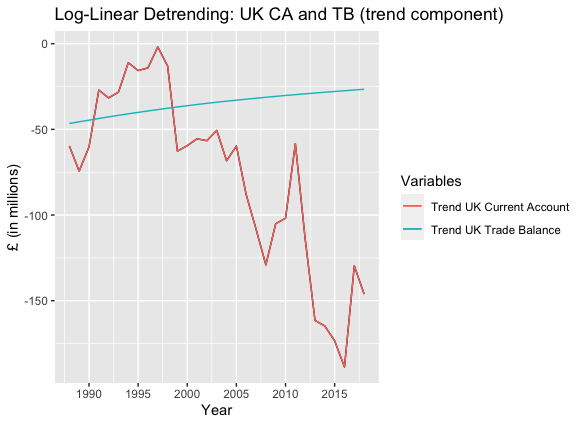
\includegraphics[scale=0.45]{11.png}
\label{}
\caption{Log-Linear Detrending: UK Current Account \\ and Trade Balance (trend component).}
\end{subfigure}%
\begin{subfigure}{.5\textwidth}
\centering
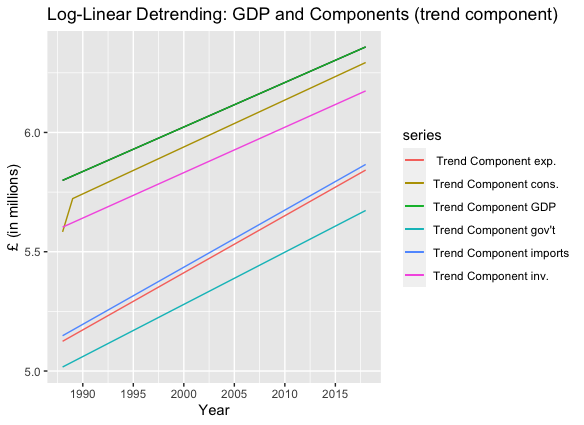
\includegraphics[scale=0.45]{10.png}
\label{}
\caption{Log-Linear Detrending: GDP and Components (trend components).}
\end{subfigure}
\end{figure}

\begin{flushleft}
Displayed above are the 'trend' components of the following variables: CA, TB, GDP, consumption, investment, government spending, net exports, and imports. 
\break
\linebreak
We can see that, with the exception of all variables except for the Current Account, all of the variables appear to be in an uptrend. GDP and its components display a clear consistent upward trend with very similar slopes. The Trade Balance, on the left figure, appears to be in an upward trend that is coming to an end (i.e. it is increasing at a decreasing rate).
\break
\linebreak
The detrended Current Account displays similar behavior to the detrended CA in the HP filter process. Although very volatile, it is clearly in a downward trend.
\end{flushleft}

\newpage

\subsection{Cyclical Components}

\begin{figure}[h!]
\centering
\begin{subfigure}{.5\textwidth}
  \centering
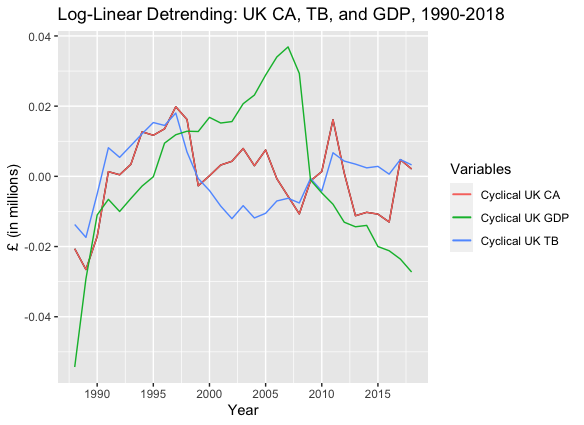
\includegraphics[scale=0.45]{6.png}
\label{}
\caption{Log-Linear Detrending: UK CA, TB, and GDP, \\ 1990-2018 (cyclical components).}
\end{subfigure}%
\begin{subfigure}{.5\textwidth}
\centering
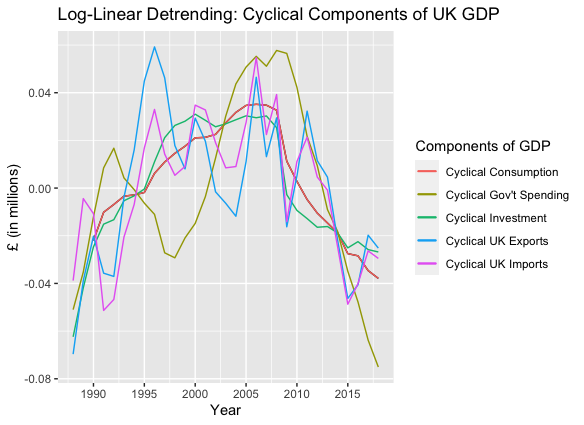
\includegraphics[scale=0.45]{7.png}
\label{}
\caption{Log-Linear Detrending: Cyclical Components of UK GDP, 1990-2018.}
\end{subfigure}
\end{figure}

\begin{flushleft}
Displayed above are the 'cyclical' components of the following variables: CA, TB, GDP, consumption, investment, government spending, net exports, and imports. 
\break
\linebreak
When observing the figures, we can see that the Current Account and Trade Balance tend to move in tandem with one another for the most part (with the exception of 1999-2008). 
\break
\linebreak
GDP and its components all move in the same direction with one another and all possess fairly similar cyclical behavior. Among these, consumption and investment appear to be the least volatile and are "smooth". It also appears that there is a negative relationship between the cyclical component of UK Exports and government expenditure.
\end{flushleft}

\newpage

\section{Log-Quadratic Detrending}

In this section, I provide a brief overview of the Log-Quaddratic detrending method that was implemented in this project. The Log-Quadratic detrending process was completed in RStudio through running a regression of logged variables on two trend variables $t$, where $t \ \epsilon \ \{1,...31\}$ and $t^2$, where $t^2 \ \epsilon \ \{1,4,9...961\}$.

\subsection{Trend Components}

\begin{figure}[h!]
\centering
\begin{subfigure}{.5\textwidth}
  \centering
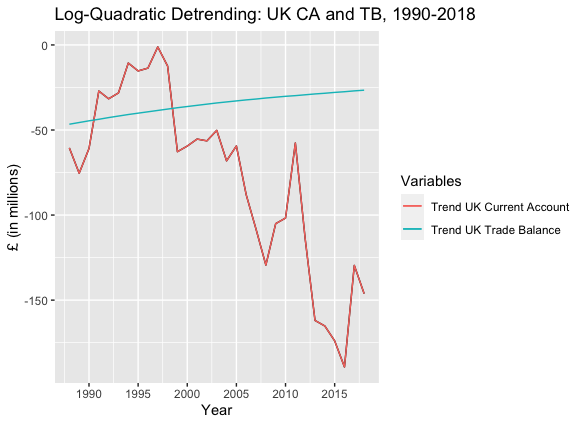
\includegraphics[scale=0.45]{13.png}
\label{}
\caption{Log-Quadratic Detrending: UK Current Account \\ and Trade Balance (trend component).}
\end{subfigure}%
\begin{subfigure}{.5\textwidth}
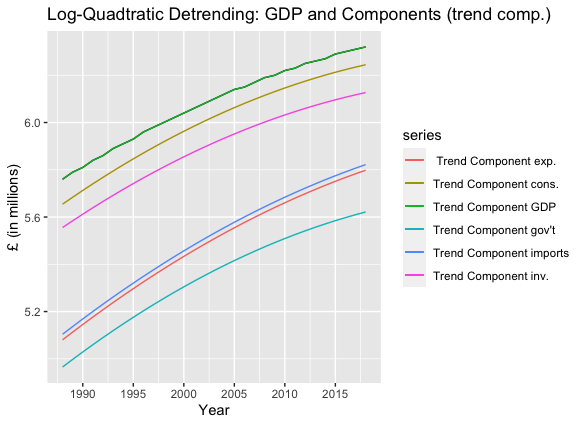
\includegraphics[scale=0.45]{12.png}
\label{}
\caption{Log-Quadtratic Detrending: GDP and Components (trend component).}
\end{subfigure}
\end{figure}

\begin{flushleft}
Displayed above are the 'trend' components of the following variables: CA, TB, GDP, consumption, investment, government spending, net exports, and imports. 
\break
\linebreak
We can see that, with the exception of all variables except for the Current Account, all of the variables appear to be in an uptrend. GDP and its components display a clear consistent upward trend with very similar slopes. The Trade Balance, on the left figure, appears to be in an upward trend that is coming to an end (i.e. it is increasing at a decreasing rate).
\break
\linebreak
The detrended Current Account displays similar behavior to the detrended CA in the HP filter process and in the Log-Linear detrending process. Although very volatile, it is clearly in a downward trend.
\end{flushleft}

\newpage

\subsection{Cyclical Components}

\begin{figure}[h!]
\centering
\begin{subfigure}{.5\textwidth}
  \centering
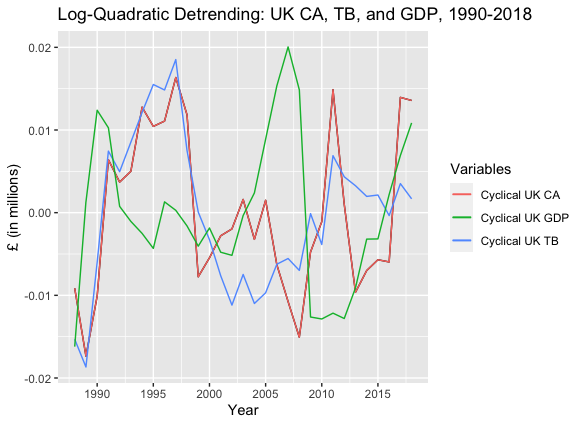
\includegraphics[scale=0.45]{8.png}
\label{}
\caption{Log-Quadratic Detrending: UK CA, TB, and \\ GDP, 1990-2018 (cyclical component).}
\end{subfigure}%
\begin{subfigure}{.5\textwidth}
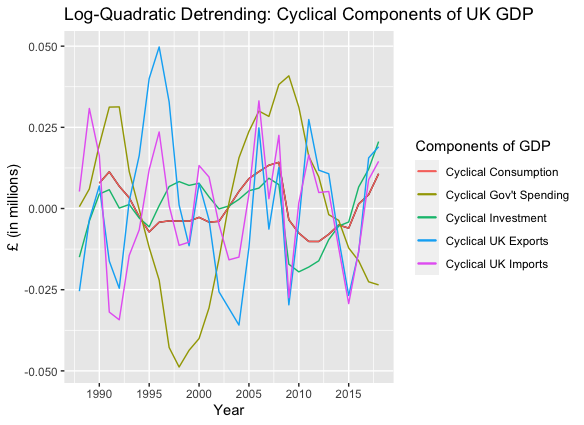
\includegraphics[scale=0.45]{9.png}
\label{}
\caption{Log-Quadratic Detrending: Cyclical Components \\ of UK GDP.}
\end{subfigure}
\end{figure}

\begin{flushleft}
Displayed above are the 'cyclical' components of the following variables: CA, TB, GDP, consumption, investment, government spending, net exports, and imports. 
\break
\linebreak
When observing the figures, we can see that the Current Account and Trade Balance tend to move in tandem with one another for the most part (with the exception of 2000-2006). 
\break
\linebreak
GDP and its components all move in the same direction with one another and all possess fairly similar cyclical behavior. Among these, consumption and investment appear to be the least volatile and are "smooth". It also appears that there is a negative relationship between the cyclical component of UK Exports and government expenditure.
\end{flushleft}

\newpage

\section{Log-Quadtratic Detrending and Business Cycle Facts}

The final section of this project deals with verifying the \textbf{Ten Facts about Business Cycles Around the World} discussed in 5P08 lecture. I use the detrended components of GDP obtained from the Log-Quadratic detrending process. I find that the behavior of GDP components, when detrended using a LQ process, display identical behavior to that observed in the Ten Business Cycle Facts.

\subsection{Standard Deviations}

\begin{table}[!htbp] \centering
\caption{Standard deviations for TB, CA, GDP, and GDP components.}
\label{}
\small
\begin{tabular}{@{\extracolsep{0.5pt}} cccccccccc}
\\[-1.8ex]\hline
\hline \\[-1.8ex]
& $\sigma_{ca}$ & $\sigma_{tb}$ &$\sigma_{y}$ & $\sigma_{c}$ & $\sigma_{i}$ & $\sigma_{g}$ & $\sigma_{x}$ & $\sigma_{m}$  \\
\hline \\[-1.8ex]
& 0.009492918	& 0.009087988	& 0.009087037 & 0.00751968 & 0.009670633 & 0.026135564 & 0.022028849 & 0.017863292  \\
\hline \\[-1.8ex]
\end{tabular}
\end{table}

The first table displays the standard deviations of each variables. We see that the standard deviations for the Current Account, Trade Balance, GDP, consumption and investment are all very small (less than 1\%). The standard deviations of government expenditure, exports, and imports are also all very small ($>3\%$). There does not appear to be a very volatile business cycle present given the small standard deviation of output. 

\subsection{Correlations with Output}

\begin{table}[!htbp] \centering
\caption{Correlations with output.}
\label{}
\small
\begin{tabular}{@{\extracolsep{0.5pt}} ccccccccc}
\\[-1.8ex]\hline
\hline \\[-1.8ex]
& $corr(ca,y)$ & $corr(tb,y)$ & $corr(c,y)$ & $corr(i,y)$ & $corr(g/y,y)$ & $corr(x,y)$ & $corr(m,y)$  \\
\hline \\[-1.8ex]
& -0.092836107 & -0.110607472 & 0.032866044& 0.794068008 & -2.31889E-11 & 0.142550988 & 0.221234394  \\
\hline \\[-1.8ex]
\end{tabular}
\end{table}

\begin{flushleft}
The next table displays the correlations of each variable with output. Here, we do see some verfication of Business Cycle Facts 4-6. 
\break
\linebreak
Fact 4 states that consumption, investment, exports, and imports are all procyclical. We can see that the correlations of $c$, $i$, $x$, and $m$ are all positive, indicating procycial behavior.
\break
\linebreak
Fact 5 states that the Trade Balance and Current account are countercyclical with output. As we can see, Fact 5 appears to hold true in the case of the UK as the correlation between TB and output and CA and output are both negative, indicating countercyclical behavior.
\break
\linebreak
Lastly, Fact 6 states that the share of government consumption in output is acyclical. In this instance, the correlation of the share of gov't consumption and ouput is very small (approximately equal to zero), thus displaying acyclical behavior.
\end{flushleft}

\newpage

\subsection{Serial Correlations}

\begin{table}[!htbp] \centering
\caption{Serial correlations.}
\label{}
\tiny
\begin{tabular}{@{\extracolsep{5pt}} cccccccccc}
\\[-1.8ex]\hline
\hline \\[-1.8ex]
& $corr(ca_t,ca_{t-1})$ & $corr(tb_t,tb_{t-1})$ & $corr(y_t,y_{t-1})$ & $corr(c_t,c_{t-1})$ & $corr(i_t,i_{t-1})$ & $corr(g_t,g_{t-1})$ & $corr(x_t,x_{t-1})$  & $corr(m_t,m_{t-1})$  \\
\hline \\[-1.8ex]
& 0.009492918	& 0.009087988	& 0.009087037 & 0.00751968 & 0.009670633 & 0.026135564 & 0.022028849 & 0.017863292  \\
\hline \\[-1.8ex]
\end{tabular}
\end{table}

The next table displays the serial correlations of every variable with itself. These figures are meant to demonstrate the validity of Fact 7, which states that all components of demand ($i$, $x$, and $m$) and supply ($y$, $m$) are positively serially correlated. We see that every single variable displays a positive serial correlation, providing evidence to the validity of Fact 7. It should be noted however that the correlations themselves are fairly small ($>1\%$).
\subsection{Output Ratios}

\begin{table}[!htbp] \centering
\caption{Output ratios.}
\label{}
\small
\begin{tabular}{@{\extracolsep{0.5pt}} ccccccccc}
\\[-1.8ex]\hline
\hline \\[-1.8ex]
& $\frac{\sigma_{ca}}{\sigma_{y}}$ & $\frac{\sigma_{tb}}{\sigma_{y}}$ & $\frac{\sigma_{c}}{\sigma_{y}}$ & $\frac{\sigma_{i}}{\sigma_{y}}$ & $\frac{\sigma_{g}}{\sigma_{y}}$ & $\frac{\sigma_{x}}{\sigma_{y}}$ & $\frac{\sigma_{m}}{\sigma_{y}}$ \\
\hline \\[-1.8ex]
& 1.044665947 & 1.000104684 & 0.827517193 & 1.064222889 & 2.876137021 & 2.424205929 & 1.965799387  \\
\hline \\[-1.8ex]
\end{tabular}
\end{table}

\begin{flushleft}
The final table displays the output ratios of each variable. Fact 3 states that the ranking of cross-country average standard deviations from top to bottom is imports, investment, exports, government spending, consumption, and ouput. As we can see from the data, the ranking of volatility is as follows: government spending, exports, imports, investment, and consumption. Thus, a verfication of Fact 3 cannot be made as it does not follow the Global Ranking of Volatilities.
\break
\linebreak
However, we can verify Fact 2, which states that private consumption is more volatile than output. Since $\frac{\sigma_{c}}{\sigma_{y}}>1$, Fact 2 appears to hold true.
\end{flushleft}

\newpage

\section{Bibliography}

\begin{flushleft}
\begin{itemize}
\item HP-Filter online:
\break
https://dge.repec.org/cgi-bin/hpfilter.cgi
\item OECD.stat:
\break
https://stats.oecd.org/index.aspx?queryid=25673\#
\item Office for National Statistics:
\break
https://www.ons.gov.uk/economy/nationalaccounts/uksectoraccounts/datasets/
https://www.ons.gov.uk/peoplepopulationandcommunity/populationandmigration/
populationestimates/timeseries/ukpop/pop
\end{itemize}
\end{flushleft}

\newpage

\section{Coding and Output}

\subsection{Coding}

\begin{verbatim}
setwd("~/Documents/NEW MAC/Office/Brock/MBE/ECON 5P08/PROJECT")

install.packages("dynlm")
install.packages("car")
install.packages("psych")
install.packages("ggplot2")
install.packages("forecast")
install.packages("fpp2")
library(dynlm)
library(car)
library(psych)
library("ggplot2")
library("forecast")
library("fpp2")

df<-read.csv("PROJECT DATA.csv", header = TRUE)

#plot GDP components
GDP_exp<- df$GDP_exp
CONS_exp<-df$CONS_exp
INV_exp<-df$INV_exp
GOVT_exp<-df$GOVT_exp
EXP_exp<-df$EXP_exp
IM_exp<-df$IM_exp
GDP_exp<- ts(GDP_exp,start=c(1988,1), end=c(2018,1))
CONS_exp<- ts(CONS_exp,start=c(1988,1), end=c(2018,1))
INV_exp<- ts(INV_exp,start=c(1988,1), end=c(2018,1))
GOVT_exp<- ts(GOVT_exp,start=c(1988,1), end=c(2018,1))
EXP_exp<- ts(EXP_exp,start=c(1988,1), end=c(2018,1))
IM_exp<- ts(IM_exp,start=c(1988,1), end=c(2018,1))
GDP_exp<-window(GDP_exp,start=c(1988,1), end=c(2018,1)) 
autoplot(GDP_exp) + autolayer(GDP_exp, series="UK GDP exp.") +
  autolayer(CONS_exp, series="UK cons. exp.") +
  autolayer(INV_exp, series="UK inv. exp.") +
  autolayer(GOVT_exp, series="UK gov't exp.") +
  autolayer(EXP_exp, series="UK export exp.") +
  autolayer(IM_exp, series="UK import exp.") +
  ggtitle("UK GDP and Components (expenditure approach), 1988-2018") + xlab("Year") + ylab("£ (in millions)")

  
#plot log GDP components
log_GDP_exp<- df$log_GDP_exp
log_CONS_exp<-df$log_CONS_exp
log_INV_exp<-df$log_INV_exp
log_GOVT_exp<-df$log_GOVT_exp
log_EXP_exp<-df$log_EXP_exp
log_IM_exp<-df$log_IM_exp
log_GDP_exp<- ts(log_GDP_exp,start=c(1988,1), end=c(2018,1))
log_CONS_exp<- ts(log_CONS_exp,start=c(1988,1), end=c(2018,1))
log_INV_exp<- ts(log_INV_exp,start=c(1988,1), end=c(2018,1))
log_GOVT_exp<- ts(log_GOVT_exp,start=c(1988,1), end=c(2018,1))
log_EXP_exp<- ts(log_EXP_exp,start=c(1988,1), end=c(2018,1))
log_IM_exp<- ts(log_IM_exp,start=c(1988,1), end=c(2018,1))
log_GDP_exp<-window(log_GDP_exp,start=c(1988,1), end=c(2018,1)) 
autoplot(log_GDP_exp) + autolayer(log_GDP_exp, series="UK GDP exp.") +
  autolayer(log_CONS_exp, series="UK cons. exp.") +
  autolayer(log_INV_exp, series="UK inv. exp.") +
  autolayer(log_GOVT_exp, series="UK gov't exp.") +
  autolayer(log_EXP_exp, series="UK export exp.") +
  autolayer(log_IM_exp, series="UK import exp.") +
  ggtitle("UK Log-GDP and Components (expenditure approach), 1988-2018") + xlab("Year") + ylab("£ (in millions)")


#plot CA
Current_Account<- df$Current_Account
Current_Account<- ts(Current_Account,start=c(1988,1), end=c(2018,1))

#plot TB
Trade_Balance<- df$Trade_Balance
Trade_Balance<- ts(Trade_Balance,start=c(1988,1), end=c(2018,1))

#plot NIIP
NIIP<-df$NIIP
NIIP<- ts(NIIP,start=c(1988,1), end=c(2018,1))

Current_Account<-window(Current_Account,start=c(1988,1), end=c(2018,1)) 
autoplot(Current_Account) + autolayer(Current_Account, series="UK Current Account") + 
  autolayer(Trade_Balance, series="UK Trade Balance") + autolayer(NIIP, series="UK NIIP") + 
  ggtitle("UK Balance of Payments Data, 1990-2018") + xlab("Year") + ylab("£ (in millions)") + guides(colour=guide_legend(title="Variables"))

#plot CA as % of GDP
Current_Account_GDP<-df$Current_Account_GDP
Current_Account_GDP<- ts(Current_Account_GDP,start=c(1988,1), end=c(2018,1))

#plot TB as % of GDP
Trade_Balance_GDP<- df$Trade_Balance_GDP
Trade_Balance_GDP<- ts(Trade_Balance_GDP,start=c(1988,1), end=c(2018,1))

Current_Account_GDP<-window(Current_Account_GDP,start=c(1988,1), end=c(2018,1)) 
autoplot(Current_Account_GDP) + autolayer(Current_Account_GDP, series="Current Account (as % of GDP)") + autolayer(Trade_Balance_GDP, series="Trade Balance (as % of GDP)") + 
  ggtitle("UK Current Acccount & Trade Balance (as % of GDP), 1988-2018") + 
  xlab("Year") + ylab("£ (in millions)") + guides(colour=guide_legend(title="Variables"))


#plot trade balance w/ EU and non -EU (missing data)
Trade_EU<-df$Trade_EU
Trade_EU<- ts(Trade_EU,start=c(1988,1), end=c(2018,1))
Trade_non_EU<-df$Trade_non_EU
Trade_non_EU<- ts(Trade_non_EU,start=c(1988,1), end=c(2018,1))
Trade_EU<-window(Trade_EU,start=c(1999,1), end=c(2018,1)) 
autoplot(Trade_EU) + autolayer(Trade_EU, series="Trade Balance w/ EU countries") + autolayer(Trade_non_EU, series="Trade Balance w/ non-EU countries") + 
  ggtitle("UK Trade Balance (EU vs.Non-EU countries), 1990-2018") + 
  xlab("Year") + ylab("Trade Balance (in millions of pounds)") + guides(colour=guide_legend(title="Bilateral Trade"))

#Plot w/ major trading partners
TB_US<-df$Trade.Balance.US
TB_US<- ts(TB_US,start=c(1988,1), end=c(2018,1))
TB_DEU<-df$Trade.Balance.Germany
TB_DEU<- ts(TB_DEU,start=c(1988,1), end=c(2018,1))
TB_NED<-df$Trade.Balance.Netherlands
TB_NED<- ts(TB_NED,start=c(1988,1), end=c(2018,1))
TB_FRA<-df$Trade.Balance.France
TB_FRA<- ts(TB_FRA,start=c(1988,1), end=c(2018,1))
TB_CHINA<-df$Trade.Balance.China
TB_CHINA<- ts(TB_CHINA,start=c(1988,1), end=c(2018,1))

US_trade<-window(TB_US,start=c(1988,1), end=c(2018,1)) 
autoplot(TB_US) + autolayer(TB_FRA, series="Trade Balance w/ France") + autolayer(TB_DEU, series="Trade Balance w/ Germany") +
  autolayer(TB_NED, series="Trade Balance w/ Netherlands") + autolayer(TB_CHINA, series="Trade Balance w/ China") + 
  autolayer(TB_US, series="Trade Balance w/ US") +
  ggtitle("UK Trade Balance with Major Trading Partners, 1990-2018") + 
  xlab("Year") + ylab("Trade Balance (in millions of pounds)") + guides(colour=guide_legend(title="Trade Partners"))

#Hp-filter

Detrended_Current_Account<-df$Detrended_Current_Account
Detrended_Trade_Balance<-df$Detrended_Trade_Balance
trend_GDP_exp_HP<-df$trend_GDP_exp_HP
trend_CONS_exp_HP<-df$trend_CONS_exp_HP
trend_INV_exp_HP<-df$trend_INV_exp_HP
trend_GOVT_exp_HP<-df$trend_GOVT_exp_HP
trend_EXP_exp_HP<-df$trend_EXP_exp_HP	
trend_IM_exp_HP<-df$trend_IM_exp_HP
Detrended_Current_Account<- ts(Detrended_Current_Account,start=c(1988,1), end=c(2018,1))
Detrended_Trade_Balance<- ts(Detrended_Trade_Balance,start=c(1988,1), end=c(2018,1))
trend_GDP_exp_HP<- ts(trend_GDP_exp_HP,start=c(1988,1), end=c(2018,1))
trend_CONS_exp_HP<- ts(trend_CONS_exp_HP,start=c(1988,1), end=c(2018,1))
trend_INV_exp_HP<- ts(trend_INV_exp_HP,start=c(1988,1), end=c(2018,1))
trend_GOVT_exp_HP<- ts(trend_GOVT_exp_HP,start=c(1988,1), end=c(2018,1))
trend_EXP_exp_HP<- ts(trend_EXP_exp_HP,start=c(1988,1), end=c(2018,1))
trend_IM_exp_HP<- ts(trend_IM_exp_HP,start=c(1988,1), end=c(2018,1))
trend_GDP_exp_HP<-window(trend_GDP_exp_HP,start=c(1988,1), end=c(2018,1)) 
autoplot(trend_GDP_exp_HP) +
  autolayer(trend_GDP_exp_HP, series="Trend Component GDP") +
  autolayer(trend_CONS_exp_HP, series="Trend Component cons.") +
  autolayer(trend_INV_exp_HP, series="Trend Component inv.") +
  autolayer(trend_GOVT_exp_HP, series="Trend Component gov't") +
  autolayer(trend_EXP_exp_HP, series=" Trend Component exp.") +
  autolayer(trend_IM_exp_HP, series="Trend Component imports") +
  ggtitle("HP Filter Detrending: GDP and Components (trend components)") + xlab("Year") + ylab("£ (in millions)")

autoplot(Detrended_Current_Account) + autolayer(Detrended_Current_Account, series="Detrended Current Account") +
  autolayer(Detrended_Trade_Balance, series="Detrended Trade Balance") +
  ggtitle("HP Filter Detrending: CA and TB, 1988-2018") + xlab("Year") + ylab("£ (in millions)")

cyc_GDP_exp_HP<-df$cyc_GDP_exp_HP
cyc_CONS_exp_HP<-df$cyc_CONS_exp_HP
cyc_INV_exp_HP<-df$cyc_INV_exp_HP
cyc_GOVT_exp_HP<-df$cyc_GOVT_exp_HP
cyc_EXP_exp_HP<-df$cyc_EXP_exp_HP
cyc_IM_exp_HP<-df$cyc_IM_exp_HP
cyc_GDP_exp_HP<- ts(cyc_GDP_exp_HP,start=c(1988,1), end=c(2018,1))
cyc_CONS_exp_HP<- ts(cyc_CONS_exp_HP,start=c(1988,1), end=c(2018,1))
cyc_INV_exp_HP<- ts(cyc_INV_exp_HP,start=c(1988,1), end=c(2018,1))
cyc_GOVT_exp_HP<- ts(cyc_GOVT_exp_HP,start=c(1988,1), end=c(2018,1))
cyc_EXP_exp_HP<- ts(cyc_EXP_exp_HP,start=c(1988,1), end=c(2018,1))
cyc_IM_exp_HP<- ts(cyc_IM_exp_HP,start=c(1988,1), end=c(2018,1))
cyc_GDP_exp_HP<-window(cyc_GDP_exp_HP,start=c(1988,1), end=c(2018,1)) 
autoplot(cyc_GDP_exp_HP) +
  autolayer(cyc_GDP_exp_HP, series="Cyc. Component GDP") +
  autolayer(cyc_CONS_exp_HP, series="Cyc. Component cons.") +
  autolayer(cyc_INV_exp_HP, series="Cyc. Component inv.") +
  autolayer(cyc_GOVT_exp_HP, series="Cyc. Component gov't") +
  autolayer(cyc_EXP_exp_HP, series=" Cyc. Component exp.") +
  autolayer(cyc_IM_exp_HP, series="Cyc. Component imports") +
  ggtitle("HP Filter Detrending: GDP and Components (cyclical component)") + xlab("Year") + ylab("£ (in millions)")

#log-detrending

#CA
Detrended_Current_Account<-df$Detrended_Current_Account
TREND<-df$TREND
Time<-df$Time
model1<-lm(Detrended_Current_Account ~ TREND)
summary(model1)
residuals<-resid(model1)
residuals<- ts(residuals,start=c(1988,1), end=c(2018,1))

#TB
Detrended_Trade_Balance<-df$Detrended_Trade_Balance
model2<-lm(Detrended_Trade_Balance ~ TREND)
summary(model2)
residuals2<-resid(model2)
residuals2<- ts(residuals2,start=c(1988,1), end=c(2018,1))

#GDP
log_GDP_exp<-df$log_GDP_exp
model3<-lm(log_GDP_exp ~ TREND)
summary(model3)
residuals3<-resid(model3)
residuals3<- ts(residuals3,start=c(1988,1), end=c(2018,1))

residuals<-window(residuals,start=c(1988,1), end=c(2018,1)) 
autoplot(residuals) + autolayer(residuals, series="Cyclical Component of UK Current Account") +
  autolayer(residuals2, series="Cyclical Component of UK Trade Balance") + autolayer(residuals3, series="Cyclical Component of UK GDP") +
  ggtitle("Log-Linear Detrending: UK CA, TB, and GDP, 1990-2018") + 
  xlab("Year") + ylab("£ (in millions)") + guides(colour=guide_legend(title="Variables"))


#CONS
log_CONS_exp<-df$log_CONS_exp
model4<-lm(log_CONS_exp ~ TREND)
summary(model4)
residuals4<-resid(model4)
residuals4<- ts(residuals4,start=c(1988,1), end=c(2018,1))

#INV
log_INV_exp<-df$log_INV_exp
model5<-lm(log_INV_exp ~ TREND)
summary(model5)
residuals5<-resid(model5)
residuals5<- ts(residuals5,start=c(1988,1), end=c(2018,1))

#GOVT
log_GOVT_exp<-df$log_GOVT_exp
model6<-lm(log_GOVT_exp ~ TREND)
summary(model6)
residuals6<-resid(model6)
residuals6<- ts(residuals6,start=c(1988,1), end=c(2018,1))

#EXP
log_EXP_exp<-df$log_EXP_exp
model7<-lm(log_EXP_exp ~ TREND)
summary(model7)
residuals7<-resid(model7)
residuals7<- ts(residuals7,start=c(1988,1), end=c(2018,1))

#IM
log_IM_exp<-df$log_IM_exp
model8<-lm(log_IM_exp ~ TREND)
summary(model8)
residuals8<-resid(model8)
residuals8<- ts(residuals8,start=c(1988,1), end=c(2018,1))

residuals4<-window(residuals4,start=c(1990,1), end=c(2018,1)) 
autoplot(residuals4) + autolayer(residuals4, series="Cyclical Consumption") + 
  autolayer(residuals5, series="Cyclical Investment") +
  autolayer(residuals6, series="Cyclical Gov't Spending") + autolayer(residuals7, series="Cyclical UK Exports") +
  autolayer(residuals8, series="Cyclical UK Imports") + ggtitle("Log-Linear Detrending: Cyclical Components of UK GDP, 1990-2018") + 
  xlab("Year") + ylab("£ (in millions)") + guides(colour=guide_legend(title="Components of GDP"))

#Quadratic log-detrending

#CA
TREND_2<-df$TREND^2
TREND_2
model9<-lm(Detrended_Current_Account ~ TREND + TREND_2)
summary(model9)
residuals9<-resid(model9)
residuals9<- ts(residuals9,start=c(1988,1), end=c(2018,1))

#TB
model10<-lm(Detrended_Trade_Balance ~ TREND + TREND_2)
summary(model10)
residuals10<-resid(model10)
residuals10<- ts(residuals10,start=c(1988,1), end=c(2018,1))

#GDP
model11<-lm(log_GDP_exp ~ TREND + TREND_2)
summary(model11)
residuals11<-resid(model11)
residuals11<- ts(residuals11,start=c(1988,1), end=c(2018,1))

residuals9<-window(residuals9,start=c(1988,1), end=c(2018,1)) 
autoplot(residuals9) + autolayer(residuals9, series="Cyclical Component of UK Current Account") +
  autolayer(residuals10, series="Cyclical Component of UK Trade Balance") + autolayer(residuals11, series="Cyclical Component of UK GDP") +
  ggtitle("Log-Quadratic Detrending: UK CA, TB, and GDP, 1990-2018") + 
  xlab("Year") + ylab("£ (in millions)") + guides(colour=guide_legend(title="Variables"))

#CONS
model12<-lm(log_CONS_exp ~ TREND + TREND_2)
summary(model12)
residuals12<-resid(model12)
residuals12<- ts(residuals12,start=c(1988,1), end=c(2018,1))

#INV
model13<-lm(log_INV_exp ~ TREND + TREND_2)
summary(model13)
residuals13<-resid(model13)
residuals13<- ts(residuals13,start=c(1988,1), end=c(2018,1))

#GOVT
model14<-lm(log_GOVT_exp ~ TREND + TREND_2)
summary(model14)
residuals14<-resid(model14)
residuals14<- ts(residuals14,start=c(1988,1), end=c(2018,1))

#EXP
model15<-lm(log_EXP_exp ~ TREND + TREND_2)
summary(model15)
residuals15<-resid(model15)
residuals15<- ts(residuals15,start=c(1988,1), end=c(2018,1))

#IM
model16<-lm(log_IM_exp ~ TREND + TREND_2)
summary(model16)
residuals16<-resid(model16)
residuals16<- ts(residuals16,start=c(1988,1), end=c(2018,1))

residuals12<-window(residuals12,start=c(1990,1), end=c(2018,1)) 
autoplot(residuals12) + autolayer(residuals12, series="Cyclical Consumption") + 
  autolayer(residuals13, series="Cyclical Investment") +
  autolayer(residuals14, series="Cyclical Gov't Spending") + autolayer(residuals15, series="Cyclical UK Exports") +
  autolayer(residuals16, series="Cyclical UK Imports") + ggtitle("Log-Quadratic Detrending: Cyclical Components of UK GDP") + 
  xlab("Year") + ylab("£ (in millions)") + guides(colour=guide_legend(title="Components of GDP"))

#TREND COMPONENTS
trend_CA_log_det<-df$trend_CA_log_det
trend_TB_log_det<-df$trend_TB_log_det
trend_GDP_log_det<-df$trend_GDP_log_det
trend_CONS_log_det<-df$trend_CONS_log_det
trend_INV_log_det<-df$trend_INV_log_det
trend_GOVT_log_det<-df$trend_GOVT_log_det
trend_EXP_log_det<-df$trend_EXP_log_det	
trend_IM_log_det<-df$trend_IM_log_det
trend_CA_log_det<- ts(trend_CA_log_det,start=c(1988,1), end=c(2018,1))
trend_TB_log_det<- ts(trend_TB_log_det,start=c(1988,1), end=c(2018,1))
trend_GDP_log_det<- ts(trend_GDP_log_det,start=c(1988,1), end=c(2018,1))
trend_CONS_log_det<- ts(trend_CONS_log_det,start=c(1988,1), end=c(2018,1))
trend_INV_log_det<- ts(trend_INV_log_det,start=c(1988,1), end=c(2018,1))
trend_GOVT_log_det<- ts(trend_GOVT_log_det,start=c(1988,1), end=c(2018,1))
trend_EXP_log_det<- ts(trend_EXP_log_det,start=c(1988,1), end=c(2018,1))
trend_IM_log_det<- ts(trend_IM_log_det,start=c(1988,1), end=c(2018,1))
trend_GDP_log_det<-window(trend_GDP_log_det,start=c(1988,1), end=c(2018,1)) 
autoplot(trend_GDP_log_det) +
  autolayer(trend_GDP_log_det, series="Trend Component GDP") +
  autolayer(trend_CONS_log_det, series="Trend Component cons.") +
  autolayer(trend_INV_log_det, series="Trend Component inv.") +
  autolayer(trend_GOVT_log_det, series="Trend Component gov't") +
  autolayer(trend_EXP_log_det, series=" Trend Component exp.") +
  autolayer(trend_IM_log_det, series="Trend Component imports") +
  ggtitle("Log-Linear Detrending: GDP and Components (trend components)") + xlab("Year") + ylab("£ (in millions)")

trend_CA_log_det<-window(trend_CA_log_det,start=c(1988,1), end=c(2018,1)) 
autoplot(trend_CA_log_det) + autolayer(trend_CA_log_det, series="Trend Component of UK Current Account") +
  autolayer(trend_TB_log_det, series="Trend Component of UK Trade Balance") +
  ggtitle("Log-Linear Detrending: UK CA, TB, and GDP (trend component)") + 
  xlab("Year") + ylab("£ (in millions)") + guides(colour=guide_legend(title="Variables"))

trend_CA_quad<-df$trend_CA_quad
trend_TB_quad<-df$trend_TB_quad
trend_GDP_quad<-df$trend_GDP_quad
trend_CONS_quad<-df$trend_CONS_quad
trend_INV_quad<-df$trend_INV_quad
trend_GOVT_quad<-df$trend_GOVT_quad
trend_EXP_quad<-df$trend_EXP_quad	
trend_IM_quad<-df$trend_IM_quad
trend_CA_quad<- ts(trend_CA_quad,start=c(1988,1), end=c(2018,1))
trend_TB_quad<- ts(trend_TB_quad,start=c(1988,1), end=c(2018,1))
trend_GDP_quad<- ts(trend_GDP_quad,start=c(1988,1), end=c(2018,1))
trend_CONS_quad<- ts(trend_CONS_quad,start=c(1988,1), end=c(2018,1))
trend_INV_quad<- ts(trend_INV_quad,start=c(1988,1), end=c(2018,1))
trend_GOVT_quad<- ts(trend_GOVT_quad,start=c(1988,1), end=c(2018,1))
trend_EXP_quad<- ts(trend_EXP_quad,start=c(1988,1), end=c(2018,1))
trend_IM_quad<- ts(trend_IM_quad,start=c(1988,1), end=c(2018,1))
trend_GDP_quad<-window(trend_GDP_quad,start=c(1988,1), end=c(2018,1)) 
autoplot(trend_GDP_quad) +
  autolayer(trend_GDP_quad, series="Trend Component GDP") +
  autolayer(trend_CONS_quad, series="Trend Component cons.") +
  autolayer(trend_INV_quad, series="Trend Component inv.") +
  autolayer(trend_GOVT_quad, series="Trend Component gov't") +
  autolayer(trend_EXP_quad, series=" Trend Component exp.") +
  autolayer(trend_IM_quad, series="Trend Component imports") +
  ggtitle("Log-Quadtratic Detrending: GDP and Components (trend)") + xlab("Year") + ylab("£ (in millions)")

trend_CA_quad<-window(trend_CA_quad,start=c(1988,1), end=c(2018,1)) 
autoplot(trend_CA_quad) + autolayer(trend_CA_quad, series="Trend Component of UK Current Account") +
  autolayer(trend_TB_quad, series="Trend Component of UK Trade Balance") +
  ggtitle("Log-Quadratic Detrending: UK CA, TB, and GDP, 1990-2018") + 
  xlab("Year") + ylab("£ (in millions)") + guides(colour=guide_legend(title="Variables"))

\end{verbatim}

\subsection{Output}

\begin{verbatim}
> setwd("~/Documents/NEW MAC/Office/Brock/MBE/ECON 5P08/PROJECT")
> install.packages("dynlm")
Error in install.packages : Updating loaded packages
> install.packages("dynlm")
trying URL 'https://cran.rstudio.com/bin/macosx/el-capitan/contrib/3.6/dynlm_0.3-6.tgz'
Content type 'application/x-gzip' length 53133 bytes (51 KB)
==================================================
downloaded 51 KB


The downloaded binary packages are in
	/var/folders/_q/6113pqk54tx8nbx6c22jwdr40000gn/T//RtmpgSND4H/downloaded_packages
> install.packages("car")
Error in install.packages : Updating loaded packages
> install.packages("car")
trying URL 'https://cran.rstudio.com/bin/macosx/el-capitan/contrib/3.6/car_3.0-7.tgz'
Content type 'application/x-gzip' length 1555217 bytes (1.5 MB)
==================================================
downloaded 1.5 MB


The downloaded binary packages are in
	/var/folders/_q/6113pqk54tx8nbx6c22jwdr40000gn/T//RtmpgSND4H/downloaded_packages
> install.packages("psych")
Error in install.packages : Updating loaded packages
> install.packages("psych")
trying URL 'https://cran.rstudio.com/bin/macosx/el-capitan/contrib/3.6/psych_1.9.12.31.tgz'
Content type 'application/x-gzip' length 3801830 bytes (3.6 MB)
==================================================
downloaded 3.6 MB


The downloaded binary packages are in
	/var/folders/_q/6113pqk54tx8nbx6c22jwdr40000gn/T//RtmpgSND4H/downloaded_packages
> install.packages("ggplot2")
Error in install.packages : Updating loaded packages
> install.packages("ggplot2")
trying URL 'https://cran.rstudio.com/bin/macosx/el-capitan/contrib/3.6/ggplot2_3.3.0.tgz'
Content type 'application/x-gzip' length 4018200 bytes (3.8 MB)
==================================================
downloaded 3.8 MB


The downloaded binary packages are in
	/var/folders/_q/6113pqk54tx8nbx6c22jwdr40000gn/T//RtmpgSND4H/downloaded_packages
> install.packages("forecast")
Error in install.packages : Updating loaded packages
> install.packages("forecast")
trying URL 'https://cran.rstudio.com/bin/macosx/el-capitan/contrib/3.6/forecast_8.11.tgz'
Content type 'application/x-gzip' length 2483677 bytes (2.4 MB)
==================================================
downloaded 2.4 MB


The downloaded binary packages are in
	/var/folders/_q/6113pqk54tx8nbx6c22jwdr40000gn/T//RtmpgSND4H/downloaded_packages
> install.packages("fpp2")
Error in install.packages : Updating loaded packages
> install.packages("fpp2")
trying URL 'https://cran.rstudio.com/bin/macosx/el-capitan/contrib/3.6/fpp2_2.3.tgz'
Content type 'application/x-gzip' length 342430 bytes (334 KB)
==================================================
downloaded 334 KB


The downloaded binary packages are in
	/var/folders/_q/6113pqk54tx8nbx6c22jwdr40000gn/T//RtmpgSND4H/downloaded_packages
> library(dynlm)
> library(car)
> library(psych)
> library("ggplot2")
> library("forecast")
> library("fpp2")
> df<-read.csv("PROJECT DATA.csv", header = TRUE)
> #plot GDP components
> GDP_exp<- df$GDP_exp
> CONS_exp<-df$CONS_exp
> INV_exp<-df$INV_exp
> GOVT_exp<-df$GOVT_exp
> EXP_exp<-df$EXP_exp
> IM_exp<-df$IM_exp
> GDP_exp<- ts(GDP_exp,start=c(1988,1), end=c(2018,1))
> CONS_exp<- ts(CONS_exp,start=c(1988,1), end=c(2018,1))
> INV_exp<- ts(INV_exp,start=c(1988,1), end=c(2018,1))
> GOVT_exp<- ts(GOVT_exp,start=c(1988,1), end=c(2018,1))
> EXP_exp<- ts(EXP_exp,start=c(1988,1), end=c(2018,1))
> IM_exp<- ts(IM_exp,start=c(1988,1), end=c(2018,1))
> GDP_exp<-window(GDP_exp,start=c(1988,1), end=c(2018,1)) 
> autoplot(GDP_exp) + autolayer(GDP_exp, series="UK GDP exp.") +
+   autolayer(CONS_exp, series="UK cons. exp.") +
+   autolayer(INV_exp, series="UK inv. exp.") +
+   autolayer(GOVT_exp, series="UK gov't exp.") +
+   autolayer(EXP_exp, series="UK export exp.") +
+   autolayer(IM_exp, series="UK import exp.") +
+   ggtitle("UK GDP and Components (expenditure approach), 1988-2018") + xlab("Year") + ylab("£ (in millions)")
> #plot log GDP components
> log_GDP_exp<- df$log_GDP_exp
> log_CONS_exp<-df$log_CONS_exp
> log_INV_exp<-df$log_INV_exp
> log_GOVT_exp<-df$log_GOVT_exp
> log_EXP_exp<-df$log_EXP_exp
> log_IM_exp<-df$log_IM_exp
> log_GDP_exp<- ts(log_GDP_exp,start=c(1988,1), end=c(2018,1))
> log_CONS_exp<- ts(log_CONS_exp,start=c(1988,1), end=c(2018,1))
> log_INV_exp<- ts(log_INV_exp,start=c(1988,1), end=c(2018,1))
> log_GOVT_exp<- ts(log_GOVT_exp,start=c(1988,1), end=c(2018,1))
> log_EXP_exp<- ts(log_EXP_exp,start=c(1988,1), end=c(2018,1))
> log_IM_exp<- ts(log_IM_exp,start=c(1988,1), end=c(2018,1))
> log_GDP_exp<-window(log_GDP_exp,start=c(1988,1), end=c(2018,1)) 
> autoplot(log_GDP_exp) + autolayer(log_GDP_exp, series="UK GDP exp.") +
+   autolayer(log_CONS_exp, series="UK cons. exp.") +
+   autolayer(log_INV_exp, series="UK inv. exp.") +
+   autolayer(log_GOVT_exp, series="UK gov't exp.") +
+   autolayer(log_EXP_exp, series="UK export exp.") +
+   autolayer(log_IM_exp, series="UK import exp.") +
+   ggtitle("UK Log-GDP and Components (expenditure approach), 1988-2018") + xlab("Year") + ylab("£ (in millions)")
> #plot CA
> Current_Account<- df$Current_Account
> Current_Account<- ts(Current_Account,start=c(1988,1), end=c(2018,1))
> #plot TB
> Trade_Balance<- df$Trade_Balance
> Trade_Balance<- ts(Trade_Balance,start=c(1988,1), end=c(2018,1))
> #plot NIIP
> NIIP<-df$NIIP
> NIIP<- ts(NIIP,start=c(1988,1), end=c(2018,1))
> Current_Account<-window(Current_Account,start=c(1988,1), end=c(2018,1)) 
> autoplot(Current_Account) + autolayer(Current_Account, series="UK Current Account") + 
+   autolayer(Trade_Balance, series="UK Trade Balance") + autolayer(NIIP, series="UK NIIP") + 
+   ggtitle("UK Balance of Payments Data, 1990-2018") + xlab("Year") + ylab("£ (in millions)") + guides(colour=guide_legend(title="Variables"))
> #plot CA as % of GDP
> Current_Account_GDP<-df$Current_Account_GDP
> Current_Account_GDP<- ts(Current_Account_GDP,start=c(1988,1), end=c(2018,1))
> #plot TB as % of GDP
> Trade_Balance_GDP<- df$Trade_Balance_GDP
> Trade_Balance_GDP<- ts(Trade_Balance_GDP,start=c(1988,1), end=c(2018,1))
> Current_Account_GDP<-window(Current_Account_GDP,start=c(1988,1), end=c(2018,1)) 
> autoplot(Current_Account_GDP) + autolayer(Current_Account_GDP, series="Current Account (as % of GDP)") + autolayer(Trade_Balance_GDP, series="Trade Balance (as % of GDP)") + 
+   ggtitle("UK Current Acccount & Trade Balance (as % of GDP), 1988-2018") + 
+   xlab("Year") + ylab("£ (in millions)") + guides(colour=guide_legend(title="Variables"))
> #plot trade balance w/ EU and non -EU (missing data)
> Trade_EU<-df$Trade_EU
> Trade_EU<- ts(Trade_EU,start=c(1988,1), end=c(2018,1))
> Trade_non_EU<-df$Trade_non_EU
> Trade_non_EU<- ts(Trade_non_EU,start=c(1988,1), end=c(2018,1))
> Trade_EU<-window(Trade_EU,start=c(1999,1), end=c(2018,1)) 
> autoplot(Trade_EU) + autolayer(Trade_EU, series="Trade Balance w/ EU countries") + autolayer(Trade_non_EU, series="Trade Balance w/ non-EU countries") + 
+   ggtitle("UK Trade Balance (EU vs.Non-EU countries), 1990-2018") + 
+   xlab("Year") + ylab("Trade Balance (in millions of pounds)") + guides(colour=guide_legend(title="Bilateral Trade"))
Warning message:
Removed 11 row(s) containing missing values (geom_path). 
> #Plot w/ major trading partners
> TB_US<-df$Trade.Balance.US
> TB_US<- ts(TB_US,start=c(1988,1), end=c(2018,1))
> TB_DEU<-df$Trade.Balance.Germany
> TB_DEU<- ts(TB_DEU,start=c(1988,1), end=c(2018,1))
> TB_NED<-df$Trade.Balance.Netherlands
> TB_NED<- ts(TB_NED,start=c(1988,1), end=c(2018,1))
> TB_FRA<-df$Trade.Balance.France
> TB_FRA<- ts(TB_FRA,start=c(1988,1), end=c(2018,1))
> TB_CHINA<-df$Trade.Balance.China
> TB_CHINA<- ts(TB_CHINA,start=c(1988,1), end=c(2018,1))
> US_trade<-window(TB_US,start=c(1988,1), end=c(2018,1)) 
> autoplot(TB_US) + autolayer(TB_FRA, series="Trade Balance w/ France") + autolayer(TB_DEU, series="Trade Balance w/ Germany") +
+   autolayer(TB_NED, series="Trade Balance w/ Netherlands") + autolayer(TB_CHINA, series="Trade Balance w/ China") + 
+   autolayer(TB_US, series="Trade Balance w/ US") +
+   ggtitle("UK Trade Balance with Major Trading Partners, 1990-2018") + 
+   xlab("Year") + ylab("Trade Balance (in millions of pounds)") + guides(colour=guide_legend(title="Trade Partners"))
Warning messages:
1: Removed 2 row(s) containing missing values (geom_path). 
2: Removed 2 row(s) containing missing values (geom_path). 
3: Removed 2 row(s) containing missing values (geom_path). 
4: Removed 2 row(s) containing missing values (geom_path). 
5: Removed 2 row(s) containing missing values (geom_path). 
> Detrended_Current_Account<-df$Detrended_Current_Account
> Detrended_Trade_Balance<-df$Detrended_Trade_Balance
> trend_GDP_exp_HP<-df$trend_GDP_exp_HP
> trend_CONS_exp_HP<-df$trend_CONS_exp_HP
> trend_INV_exp_HP<-df$trend_INV_exp_HP
> trend_GOVT_exp_HP<-df$trend_GOVT_exp_HP
> trend_EXP_exp_HP<-df$trend_EXP_exp_HP	
> trend_IM_exp_HP<-df$trend_IM_exp_HP
> Detrended_Current_Account<- ts(Detrended_Current_Account,start=c(1988,1), end=c(2018,1))
> Detrended_Trade_Balance<- ts(Detrended_Trade_Balance,start=c(1988,1), end=c(2018,1))
> trend_GDP_exp_HP<- ts(trend_GDP_exp_HP,start=c(1988,1), end=c(2018,1))
> trend_CONS_exp_HP<- ts(trend_CONS_exp_HP,start=c(1988,1), end=c(2018,1))
> trend_INV_exp_HP<- ts(trend_INV_exp_HP,start=c(1988,1), end=c(2018,1))
> trend_GOVT_exp_HP<- ts(trend_GOVT_exp_HP,start=c(1988,1), end=c(2018,1))
> trend_EXP_exp_HP<- ts(trend_EXP_exp_HP,start=c(1988,1), end=c(2018,1))
> trend_IM_exp_HP<- ts(trend_IM_exp_HP,start=c(1988,1), end=c(2018,1))
> trend_GDP_exp_HP<-window(trend_GDP_exp_HP,start=c(1988,1), end=c(2018,1)) 
> autoplot(trend_GDP_exp_HP) +
+   autolayer(trend_GDP_exp_HP, series="Trend Component GDP") +
+   autolayer(trend_CONS_exp_HP, series="Trend Component cons.") +
+   autolayer(trend_INV_exp_HP, series="Trend Component inv.") +
+   autolayer(trend_GOVT_exp_HP, series="Trend Component gov't") +
+   autolayer(trend_EXP_exp_HP, series=" Trend Component exp.") +
+   autolayer(trend_IM_exp_HP, series="Trend Component imports") +
+   ggtitle("HP Filter Detrending: GDP and Components (trend components)") + xlab("Year") + ylab("£ (in millions)")
> autoplot(Detrended_Current_Account) + autolayer(Detrended_Current_Account, series="Detrended Current Account") +
+   autolayer(Detrended_Trade_Balance, series="Detrended Trade Balance") +
+   ggtitle("HP Filter Detrending: CA and TB, 1988-2018") + xlab("Year") + ylab("£ (in millions)")
> cyc_GDP_exp_HP<-df$cyc_GDP_exp_HP
> cyc_CONS_exp_HP<-df$cyc_CONS_exp_HP
> cyc_INV_exp_HP<-df$cyc_INV_exp_HP
> cyc_GOVT_exp_HP<-df$cyc_GOVT_exp_HP
> cyc_EXP_exp_HP<-df$cyc_EXP_exp_HP
> cyc_IM_exp_HP<-df$cyc_IM_exp_HP
> cyc_GDP_exp_HP<- ts(cyc_GDP_exp_HP,start=c(1988,1), end=c(2018,1))
> cyc_CONS_exp_HP<- ts(cyc_CONS_exp_HP,start=c(1988,1), end=c(2018,1))
> cyc_INV_exp_HP<- ts(cyc_INV_exp_HP,start=c(1988,1), end=c(2018,1))
> cyc_GOVT_exp_HP<- ts(cyc_GOVT_exp_HP,start=c(1988,1), end=c(2018,1))
> cyc_EXP_exp_HP<- ts(cyc_EXP_exp_HP,start=c(1988,1), end=c(2018,1))
> cyc_IM_exp_HP<- ts(cyc_IM_exp_HP,start=c(1988,1), end=c(2018,1))
> cyc_GDP_exp_HP<-window(cyc_GDP_exp_HP,start=c(1988,1), end=c(2018,1)) 
> autoplot(cyc_GDP_exp_HP) +
+   autolayer(cyc_GDP_exp_HP, series="Cyc. Component GDP") +
+   autolayer(cyc_CONS_exp_HP, series="Cyc. Component cons.") +
+   autolayer(cyc_INV_exp_HP, series="Cyc. Component inv.") +
+   autolayer(cyc_GOVT_exp_HP, series="Cyc. Component gov't") +
+   autolayer(cyc_EXP_exp_HP, series=" Cyc. Component exp.") +
+   autolayer(cyc_IM_exp_HP, series="Cyc. Component imports") +
+   ggtitle("HP Filter Detrending: GDP and Components (cyclical component)") + xlab("Year") + ylab("£ (in millions)")
> #CA
> Detrended_Current_Account<-df$Detrended_Current_Account
> TREND<-df$TREND
> Time<-df$Time
> model1<-lm(Detrended_Current_Account ~ TREND)
> summary(model1)

Call:
lm(formula = Detrended_Current_Account ~ TREND)

Residuals:
      Min        1Q    Median        3Q       Max 
-0.026549 -0.007967  0.001333  0.006139  0.019835 

Coefficients:
              Estimate Std. Error t value Pr(>|t|)    
(Intercept) -0.0109616  0.0041553  -2.638 0.013269 *  
TREND       -0.0009352  0.0002267  -4.126 0.000284 ***
---
Signif. codes:  0 ‘***’ 0.001 ‘**’ 0.01 ‘*’ 0.05 ‘.’ 0.1 ‘ ’ 1

Residual standard error: 0.01129 on 29 degrees of freedom
  (90 observations deleted due to missingness)
Multiple R-squared:  0.3698,	Adjusted R-squared:  0.3481 
F-statistic: 17.02 on 1 and 29 DF,  p-value: 0.0002842

> residuals<-resid(model1)
> residuals<- ts(residuals,start=c(1988,1), end=c(2018,1))
> #TB
> Detrended_Trade_Balance<-df$Detrended_Trade_Balance
> model2<-lm(Detrended_Trade_Balance ~ TREND)
> summary(model2)

Call:
lm(formula = Detrended_Trade_Balance ~ TREND)

Residuals:
       Min         1Q     Median         3Q        Max 
-0.0173966 -0.0073013  0.0006244  0.0060623  0.0180367 

Coefficients:
              Estimate Std. Error t value Pr(>|t|)   
(Intercept) -0.0111321  0.0034154  -3.259  0.00285 **
TREND       -0.0001853  0.0001863  -0.994  0.32825   
---
Signif. codes:  0 ‘***’ 0.001 ‘**’ 0.01 ‘*’ 0.05 ‘.’ 0.1 ‘ ’ 1

Residual standard error: 0.009279 on 29 degrees of freedom
  (90 observations deleted due to missingness)
Multiple R-squared:  0.03297,	Adjusted R-squared:  -0.0003722 
F-statistic: 0.9888 on 1 and 29 DF,  p-value: 0.3283

> residuals2<-resid(model2)
> residuals2<- ts(residuals2,start=c(1988,1), end=c(2018,1))
> #GDP
> log_GDP_exp<-df$log_GDP_exp
> model3<-lm(log_GDP_exp ~ TREND)
> summary(model3)

Call:
lm(formula = log_GDP_exp ~ TREND)

Residuals:
     Min       1Q   Median       3Q      Max 
-0.05432 -0.01352 -0.00277  0.01540  0.03687 

Coefficients:
             Estimate Std. Error t value Pr(>|t|)    
(Intercept) 5.7804276  0.0079156  730.26   <2e-16 ***
TREND       0.0186489  0.0004318   43.19   <2e-16 ***
---
Signif. codes:  0 ‘***’ 0.001 ‘**’ 0.01 ‘*’ 0.05 ‘.’ 0.1 ‘ ’ 1

Residual standard error: 0.0215 on 29 degrees of freedom
  (90 observations deleted due to missingness)
Multiple R-squared:  0.9847,	Adjusted R-squared:  0.9842 
F-statistic:  1865 on 1 and 29 DF,  p-value: < 2.2e-16

> residuals3<-resid(model3)
> residuals3<- ts(residuals3,start=c(1988,1), end=c(2018,1))
> residuals<-window(residuals,start=c(1988,1), end=c(2018,1)) 
> autoplot(residuals) + autolayer(residuals, series="Cyclical Component of UK Current Account") +
+   autolayer(residuals2, series="Cyclical Component of UK Trade Balance") + autolayer(residuals3, series="Cyclical Component of UK GDP") +
+   ggtitle("Log-Linear Detrending: UK CA, TB, and GDP, 1990-2018") + 
+   xlab("Year") + ylab("£ (in millions)") + guides(colour=guide_legend(title="Variables"))
> #CONS
> log_CONS_exp<-df$log_CONS_exp
> model4<-lm(log_CONS_exp ~ TREND)
> summary(model4)

Call:
lm(formula = log_CONS_exp ~ TREND)

Residuals:
      Min        1Q    Median        3Q       Max 
-0.059931 -0.016726 -0.001851  0.021178  0.035143 

Coefficients:
             Estimate Std. Error t value Pr(>|t|)    
(Intercept) 5.6834303  0.0095367  595.95   <2e-16 ***
TREND       0.0196705  0.0005203   37.81   <2e-16 ***
---
Signif. codes:  0 ‘***’ 0.001 ‘**’ 0.01 ‘*’ 0.05 ‘.’ 0.1 ‘ ’ 1

Residual standard error: 0.02591 on 29 degrees of freedom
  (90 observations deleted due to missingness)
Multiple R-squared:  0.9801,	Adjusted R-squared:  0.9794 
F-statistic:  1429 on 1 and 29 DF,  p-value: < 2.2e-16

> residuals4<-resid(model4)
> residuals4<- ts(residuals4,start=c(1988,1), end=c(2018,1))
> #INV
> log_INV_exp<-df$log_INV_exp
> model5<-lm(log_INV_exp ~ TREND)
> summary(model5)

Call:
lm(formula = log_INV_exp ~ TREND)

Residuals:
      Min        1Q    Median        3Q       Max 
-0.062390 -0.017616 -0.003259  0.026617  0.030994 

Coefficients:
             Estimate Std. Error t value Pr(>|t|)    
(Intercept) 5.5840334  0.0095993  581.71   <2e-16 ***
TREND       0.0190367  0.0005237   36.35   <2e-16 ***
---
Signif. codes:  0 ‘***’ 0.001 ‘**’ 0.01 ‘*’ 0.05 ‘.’ 0.1 ‘ ’ 1

Residual standard error: 0.02608 on 29 degrees of freedom
  (90 observations deleted due to missingness)
Multiple R-squared:  0.9785,	Adjusted R-squared:  0.9778 
F-statistic:  1321 on 1 and 29 DF,  p-value: < 2.2e-16

> residuals5<-resid(model5)
> residuals5<- ts(residuals5,start=c(1988,1), end=c(2018,1))
> #GOVT
> log_GOVT_exp<-df$log_GOVT_exp
> model6<-lm(log_GOVT_exp ~ TREND)
> summary(model6)

Call:
lm(formula = log_GOVT_exp ~ TREND)

Residuals:
     Min       1Q   Median       3Q      Max 
-0.07506 -0.02403 -0.00358  0.02595  0.05773 

Coefficients:
             Estimate Std. Error t value Pr(>|t|)    
(Intercept) 4.9949385  0.0137525  363.20   <2e-16 ***
TREND       0.0218732  0.0007503   29.15   <2e-16 ***
---
Signif. codes:  0 ‘***’ 0.001 ‘**’ 0.01 ‘*’ 0.05 ‘.’ 0.1 ‘ ’ 1

Residual standard error: 0.03736 on 29 degrees of freedom
  (90 observations deleted due to missingness)
Multiple R-squared:  0.967,	Adjusted R-squared:  0.9659 
F-statistic:   850 on 1 and 29 DF,  p-value: < 2.2e-16

> residuals6<-resid(model6)
> residuals6<- ts(residuals6,start=c(1988,1), end=c(2018,1))
> #EXP
> log_EXP_exp<-df$log_EXP_exp
> model7<-lm(log_EXP_exp ~ TREND)
> summary(model7)

Call:
lm(formula = log_EXP_exp ~ TREND)

Residuals:
      Min        1Q    Median        3Q       Max 
-0.069660 -0.021007  0.004604  0.018743  0.059215 

Coefficients:
             Estimate Std. Error t value Pr(>|t|)    
(Intercept) 5.1006442  0.0116922  436.24   <2e-16 ***
TREND       0.0239277  0.0006379   37.51   <2e-16 ***
---
Signif. codes:  0 ‘***’ 0.001 ‘**’ 0.01 ‘*’ 0.05 ‘.’ 0.1 ‘ ’ 1

Residual standard error: 0.03177 on 29 degrees of freedom
  (90 observations deleted due to missingness)
Multiple R-squared:  0.9798,	Adjusted R-squared:  0.9791 
F-statistic:  1407 on 1 and 29 DF,  p-value: < 2.2e-16

> residuals7<-resid(model7)
> residuals7<- ts(residuals7,start=c(1988,1), end=c(2018,1))
> #IM
> log_IM_exp<-df$log_IM_exp
> model8<-lm(log_IM_exp ~ TREND)
> summary(model8)

Call:
lm(formula = log_IM_exp ~ TREND)

Residuals:
      Min        1Q    Median        3Q       Max 
-0.051331 -0.022591  0.005355  0.020196  0.054708 

Coefficients:
             Estimate Std. Error t value Pr(>|t|)    
(Intercept) 5.1239946  0.0106251  482.25   <2e-16 ***
TREND       0.0239357  0.0005796   41.29   <2e-16 ***
---
Signif. codes:  0 ‘***’ 0.001 ‘**’ 0.01 ‘*’ 0.05 ‘.’ 0.1 ‘ ’ 1

Residual standard error: 0.02887 on 29 degrees of freedom
  (90 observations deleted due to missingness)
Multiple R-squared:  0.9833,	Adjusted R-squared:  0.9827 
F-statistic:  1705 on 1 and 29 DF,  p-value: < 2.2e-16

> residuals8<-resid(model8)
> residuals8<- ts(residuals8,start=c(1988,1), end=c(2018,1))
> residuals4<-window(residuals4,start=c(1990,1), end=c(2018,1)) 
> autoplot(residuals4) + autolayer(residuals4, series="Cyclical Consumption") + 
+   autolayer(residuals5, series="Cyclical Investment") +
+   autolayer(residuals6, series="Cyclical Gov't Spending") + autolayer(residuals7, series="Cyclical UK Exports") +
+   autolayer(residuals8, series="Cyclical UK Imports") + ggtitle("Log-Linear Detrending: Cyclical Components of UK GDP, 1990-2018") + 
+   xlab("Year") + ylab("£ (in millions)") + guides(colour=guide_legend(title="Components of GDP"))
> #CA
> TREND_2<-df$TREND^2
> TREND_2
  [1]   1   4   9  16  25  36  49  64  81 100 121 144 169 196 225 256 289 324 361 400 441 484 529 576 625
 [26] 676 729 784 841 900 961  NA  NA  NA  NA  NA  NA  NA  NA  NA  NA  NA  NA  NA  NA  NA  NA  NA  NA  NA
 [51]  NA  NA  NA  NA  NA  NA  NA  NA  NA  NA  NA  NA  NA  NA  NA  NA  NA  NA  NA  NA  NA  NA  NA  NA  NA
 [76]  NA  NA  NA  NA  NA  NA  NA  NA  NA  NA  NA  NA  NA  NA  NA  NA  NA  NA  NA  NA  NA  NA  NA  NA  NA
[101]  NA  NA  NA  NA  NA  NA  NA  NA  NA  NA  NA  NA  NA  NA  NA  NA  NA  NA  NA  NA  NA
> model9<-lm(Detrended_Current_Account ~ TREND + TREND_2)
> summary(model9)

Call:
lm(formula = Detrended_Current_Account ~ TREND + TREND_2)

Residuals:
      Min        1Q    Median        3Q       Max 
-0.017362 -0.006652 -0.001967  0.008419  0.016350 

Coefficients:
              Estimate Std. Error t value Pr(>|t|)    
(Intercept) -2.490e-02  5.655e-03  -4.403 0.000142 ***
TREND        1.599e-03  8.147e-04   1.963 0.059705 .  
TREND_2     -7.919e-05  2.470e-05  -3.206 0.003355 ** 
---
Signif. codes:  0 ‘***’ 0.001 ‘**’ 0.01 ‘*’ 0.05 ‘.’ 0.1 ‘ ’ 1

Residual standard error: 0.009826 on 28 degrees of freedom
  (90 observations deleted due to missingness)
Multiple R-squared:  0.539,	Adjusted R-squared:  0.5061 
F-statistic: 16.37 on 2 and 28 DF,  p-value: 1.956e-05

> residuals9<-resid(model9)
> residuals9<- ts(residuals9,start=c(1988,1), end=c(2018,1))
> #TB
> model10<-lm(Detrended_Trade_Balance ~ TREND + TREND_2)
> summary(model10)

Call:
lm(formula = Detrended_Trade_Balance ~ TREND + TREND_2)

Residuals:
       Min         1Q     Median         3Q        Max 
-0.0186704 -0.0066095  0.0000739  0.0059250  0.0185198 

Coefficients:
              Estimate Std. Error t value Pr(>|t|)
(Intercept) -9.199e-03  5.414e-03  -1.699    0.100
TREND       -5.367e-04  7.800e-04  -0.688    0.497
TREND_2      1.098e-05  2.365e-05   0.464    0.646

Residual standard error: 0.009407 on 28 degrees of freedom
  (90 observations deleted due to missingness)
Multiple R-squared:  0.04036,	Adjusted R-squared:  -0.02818 
F-statistic: 0.5889 on 2 and 28 DF,  p-value: 0.5617

> residuals10<-resid(model10)
> residuals10<- ts(residuals10,start=c(1988,1), end=c(2018,1))
> #GDP
> model11<-lm(log_GDP_exp ~ TREND + TREND_2)
> summary(model11)

Call:
lm(formula = log_GDP_exp ~ TREND + TREND_2)

Residuals:
      Min        1Q    Median        3Q       Max 
-0.016204 -0.004555 -0.001057  0.004653  0.020050 

Coefficients:
              Estimate Std. Error t value Pr(>|t|)    
(Intercept)  5.734e+00  5.414e-03 1059.21  < 2e-16 ***
TREND        2.706e-02  7.799e-04   34.70  < 2e-16 ***
TREND_2     -2.629e-04  2.365e-05  -11.12 8.84e-12 ***
---
Signif. codes:  0 ‘***’ 0.001 ‘**’ 0.01 ‘*’ 0.05 ‘.’ 0.1 ‘ ’ 1

Residual standard error: 0.009406 on 28 degrees of freedom
  (90 observations deleted due to missingness)
Multiple R-squared:  0.9972,	Adjusted R-squared:  0.997 
F-statistic:  4936 on 2 and 28 DF,  p-value: < 2.2e-16

> residuals11<-resid(model11)
> residuals11<- ts(residuals11,start=c(1988,1), end=c(2018,1))
> residuals9<-window(residuals9,start=c(1988,1), end=c(2018,1)) 
> autoplot(residuals9) + autolayer(residuals9, series="Cyclical Component of UK Current Account") +
+   autolayer(residuals10, series="Cyclical Component of UK Trade Balance") + autolayer(residuals11, series="Cyclical Component of UK GDP") +
+   ggtitle("Log-Quadratic Detrending: UK CA, TB, and GDP, 1990-2018") + 
+   xlab("Year") + ylab("£ (in millions)") + guides(colour=guide_legend(title="Variables"))
> #CONS
> model12<-lm(log_CONS_exp ~ TREND + TREND_2)
> summary(model12)

Call:
lm(formula = log_CONS_exp ~ TREND + TREND_2)

Residuals:
      Min        1Q    Median        3Q       Max 
-0.011337 -0.004652 -0.002717  0.006069  0.014223 

Coefficients:
              Estimate Std. Error t value Pr(>|t|)    
(Intercept)  5.624e+00  4.480e-03 1255.50  < 2e-16 ***
TREND        3.039e-02  6.454e-04   47.10  < 2e-16 ***
TREND_2     -3.351e-04  1.957e-05  -17.13 2.27e-16 ***
---
Signif. codes:  0 ‘***’ 0.001 ‘**’ 0.01 ‘*’ 0.05 ‘.’ 0.1 ‘ ’ 1

Residual standard error: 0.007784 on 28 degrees of freedom
  (90 observations deleted due to missingness)
Multiple R-squared:  0.9983,	Adjusted R-squared:  0.9981 
F-statistic:  8066 on 2 and 28 DF,  p-value: < 2.2e-16

> residuals12<-resid(model12)
> residuals12<- ts(residuals12,start=c(1988,1), end=c(2018,1))
> #INV
> model13<-lm(log_INV_exp ~ TREND + TREND_2)
> summary(model13)

Call:
lm(formula = log_INV_exp ~ TREND + TREND_2)

Residuals:
      Min        1Q    Median        3Q       Max 
-0.019504 -0.004775  0.001237  0.006695  0.020610 

Coefficients:
              Estimate Std. Error t value Pr(>|t|)    
(Intercept)  5.526e+00  5.761e-03  959.25  < 2e-16 ***
TREND        2.950e-02  8.300e-04   35.54  < 2e-16 ***
TREND_2     -3.270e-04  2.517e-05  -12.99 2.23e-13 ***
---
Signif. codes:  0 ‘***’ 0.001 ‘**’ 0.01 ‘*’ 0.05 ‘.’ 0.1 ‘ ’ 1

Residual standard error: 0.01001 on 28 degrees of freedom
  (90 observations deleted due to missingness)
Multiple R-squared:  0.9969,	Adjusted R-squared:  0.9967 
F-statistic:  4569 on 2 and 28 DF,  p-value: < 2.2e-16

> residuals13<-resid(model13)
> residuals13<- ts(residuals13,start=c(1988,1), end=c(2018,1))
> #GOVT
> model14<-lm(log_GOVT_exp ~ TREND + TREND_2)
> summary(model14)

Call:
lm(formula = log_GOVT_exp ~ TREND + TREND_2)

Residuals:
      Min        1Q    Median        3Q       Max 
-0.048807 -0.019074  0.000556  0.021672  0.040858 

Coefficients:
              Estimate Std. Error t value Pr(>|t|)    
(Intercept)  4.932e+00  1.557e-02 316.782  < 2e-16 ***
TREND        3.325e-02  2.243e-03  14.822 8.79e-15 ***
TREND_2     -3.554e-04  6.801e-05  -5.226 1.49e-05 ***
---
Signif. codes:  0 ‘***’ 0.001 ‘**’ 0.01 ‘*’ 0.05 ‘.’ 0.1 ‘ ’ 1

Residual standard error: 0.02705 on 28 degrees of freedom
  (90 observations deleted due to missingness)
Multiple R-squared:  0.9833,	Adjusted R-squared:  0.9821 
F-statistic: 824.3 on 2 and 28 DF,  p-value: < 2.2e-16

> residuals14<-resid(model14)
> residuals14<- ts(residuals14,start=c(1988,1), end=c(2018,1))
> #EXP
> model15<-lm(log_EXP_exp ~ TREND + TREND_2)
> summary(model15)

Call:
lm(formula = log_EXP_exp ~ TREND + TREND_2)

Residuals:
      Min        1Q    Median        3Q       Max 
-0.035901 -0.014822 -0.003448  0.014138  0.049764 

Coefficients:
              Estimate Std. Error t value Pr(>|t|)    
(Intercept)  5.047e+00  1.312e-02 384.571  < 2e-16 ***
TREND        3.368e-02  1.891e-03  17.815  < 2e-16 ***
TREND_2     -3.049e-04  5.732e-05  -5.318 1.16e-05 ***
---
Signif. codes:  0 ‘***’ 0.001 ‘**’ 0.01 ‘*’ 0.05 ‘.’ 0.1 ‘ ’ 1

Residual standard error: 0.0228 on 28 degrees of freedom
  (90 observations deleted due to missingness)
Multiple R-squared:   0.99,	Adjusted R-squared:  0.9892 
F-statistic:  1380 on 2 and 28 DF,  p-value: < 2.2e-16

> residuals15<-resid(model15)
> residuals15<- ts(residuals15,start=c(1988,1), end=c(2018,1))
> #IM
> model16<-lm(log_IM_exp ~ TREND + TREND_2)
> summary(model16)

Call:
lm(formula = log_IM_exp ~ TREND + TREND_2)

Residuals:
      Min        1Q    Median        3Q       Max 
-0.034270 -0.012649  0.003014  0.012611  0.033146 

Coefficients:
              Estimate Std. Error t value Pr(>|t|)    
(Intercept)  5.071e+00  1.064e-02 476.463  < 2e-16 ***
TREND        3.365e-02  1.533e-03  21.951  < 2e-16 ***
TREND_2     -3.037e-04  4.648e-05  -6.533 4.42e-07 ***
---
Signif. codes:  0 ‘***’ 0.001 ‘**’ 0.01 ‘*’ 0.05 ‘.’ 0.1 ‘ ’ 1

Residual standard error: 0.01849 on 28 degrees of freedom
  (90 observations deleted due to missingness)
Multiple R-squared:  0.9934,	Adjusted R-squared:  0.9929 
F-statistic:  2099 on 2 and 28 DF,  p-value: < 2.2e-16

> residuals16<-resid(model16)
> residuals16<- ts(residuals16,start=c(1988,1), end=c(2018,1))
> residuals12<-window(residuals12,start=c(1990,1), end=c(2018,1)) 
> autoplot(residuals12) + autolayer(residuals12, series="Cyclical Consumption") + 
+   autolayer(residuals13, series="Cyclical Investment") +
+   autolayer(residuals14, series="Cyclical Gov't Spending") + autolayer(residuals15, series="Cyclical UK Exports") +
+   autolayer(residuals16, series="Cyclical UK Imports") + ggtitle("Log-Quadratic Detrending: Cyclical Components of UK GDP") + 
+   xlab("Year") + ylab("£ (in millions)") + guides(colour=guide_legend(title="Components of GDP"))
> #TREND COMPONENTS
> trend_CA_log_det<-df$trend_CA_log_det
> trend_TB_log_det<-df$trend_TB_log_det
> trend_GDP_log_det<-df$trend_GDP_log_det
> trend_CONS_log_det<-df$trend_CONS_log_det
> trend_INV_log_det<-df$trend_INV_log_det
> trend_GOVT_log_det<-df$trend_GOVT_log_det
> trend_EXP_log_det<-df$trend_EXP_log_det	
> trend_IM_log_det<-df$trend_IM_log_det
> trend_CA_log_det<- ts(trend_CA_log_det,start=c(1988,1), end=c(2018,1))
> trend_TB_log_det<- ts(trend_TB_log_det,start=c(1988,1), end=c(2018,1))
> trend_GDP_log_det<- ts(trend_GDP_log_det,start=c(1988,1), end=c(2018,1))
> trend_CONS_log_det<- ts(trend_CONS_log_det,start=c(1988,1), end=c(2018,1))
> trend_INV_log_det<- ts(trend_INV_log_det,start=c(1988,1), end=c(2018,1))
> trend_GOVT_log_det<- ts(trend_GOVT_log_det,start=c(1988,1), end=c(2018,1))
> trend_EXP_log_det<- ts(trend_EXP_log_det,start=c(1988,1), end=c(2018,1))
> trend_IM_log_det<- ts(trend_IM_log_det,start=c(1988,1), end=c(2018,1))
> trend_GDP_log_det<-window(trend_GDP_log_det,start=c(1988,1), end=c(2018,1)) 
> autoplot(trend_GDP_log_det) +
+   autolayer(trend_GDP_log_det, series="Trend Component GDP") +
+   autolayer(trend_CONS_log_det, series="Trend Component cons.") +
+   autolayer(trend_INV_log_det, series="Trend Component inv.") +
+   autolayer(trend_GOVT_log_det, series="Trend Component gov't") +
+   autolayer(trend_EXP_log_det, series=" Trend Component exp.") +
+   autolayer(trend_IM_log_det, series="Trend Component imports") +
+   ggtitle("Log-Linear Detrending: GDP and Components (trend components)") + xlab("Year") + ylab("£ (in millions)")
> trend_CA_log_det<-window(trend_CA_log_det,start=c(1988,1), end=c(2018,1)) 
> autoplot(trend_CA_log_det) + autolayer(trend_CA_log_det, series="Trend Component of UK Current Account") +
+   autolayer(trend_TB_log_det, series="Trend Component of UK Trade Balance") +
+   ggtitle("Log-Linear Detrending: UK CA, TB, and GDP (trend component)") + 
+   xlab("Year") + ylab("£ (in millions)") + guides(colour=guide_legend(title="Variables"))
> trend_CA_quad<-df$trend_CA_quad
> trend_TB_quad<-df$trend_TB_quad
> trend_GDP_quad<-df$trend_GDP_quad
> trend_CONS_quad<-df$trend_CONS_quad
> trend_INV_quad<-df$trend_INV_quad
> trend_GOVT_quad<-df$trend_GOVT_quad
> trend_EXP_quad<-df$trend_EXP_quad	
> trend_IM_quad<-df$trend_IM_quad
> trend_CA_quad<- ts(trend_CA_quad,start=c(1988,1), end=c(2018,1))
> trend_TB_quad<- ts(trend_TB_quad,start=c(1988,1), end=c(2018,1))
> trend_GDP_quad<- ts(trend_GDP_quad,start=c(1988,1), end=c(2018,1))
> trend_CONS_quad<- ts(trend_CONS_quad,start=c(1988,1), end=c(2018,1))
> trend_INV_quad<- ts(trend_INV_quad,start=c(1988,1), end=c(2018,1))
> trend_GOVT_quad<- ts(trend_GOVT_quad,start=c(1988,1), end=c(2018,1))
> trend_EXP_quad<- ts(trend_EXP_quad,start=c(1988,1), end=c(2018,1))
> trend_IM_quad<- ts(trend_IM_quad,start=c(1988,1), end=c(2018,1))
> trend_GDP_quad<-window(trend_GDP_quad,start=c(1988,1), end=c(2018,1)) 
> autoplot(trend_GDP_quad) +
+   autolayer(trend_GDP_quad, series="Trend Component GDP") +
+   autolayer(trend_CONS_quad, series="Trend Component cons.") +
+   autolayer(trend_INV_quad, series="Trend Component inv.") +
+   autolayer(trend_GOVT_quad, series="Trend Component gov't") +
+   autolayer(trend_EXP_quad, series=" Trend Component exp.") +
+   autolayer(trend_IM_quad, series="Trend Component imports") +
+   ggtitle("Log-Quadtratic Detrending: GDP and Components (trend)") + xlab("Year") + ylab("£ (in millions)")
> trend_CA_quad<-window(trend_CA_quad,start=c(1988,1), end=c(2018,1)) 
> autoplot(trend_CA_quad) + autolayer(trend_CA_quad, series="Trend Component of UK Current Account") +
+   autolayer(trend_TB_quad, series="Trend Component of UK Trade Balance") +
+   ggtitle("Log-Quadratic Detrending: UK CA, TB, and GDP, 1990-2018") + 
+   xlab("Year") + ylab("£ (in millions)") + guides(colour=guide_legend(title="Variables"))
\end{verbatim}











\end{document}